\documentclass[12pt,letterpaper]{report}

\usepackage[utf8]{inputenc}
\usepackage[T1]{fontenc}
\usepackage[spanish,es-noindentfirst]{babel}
\usepackage[margin=2.5cm]{geometry}
\usepackage{hyperref}
\usepackage{enumitem}
\usepackage{amsmath}
\usepackage{graphicx}
\usepackage{titlesec}
\usepackage{xcolor}
\usepackage{booktabs}
\usepackage{float}

\hypersetup{
    colorlinks=true,
    linkcolor=black,
    citecolor=black,
    urlcolor=blue,
    pdftitle={Bitácora Co-MIL - Parte III},
    pdfauthor={Adrián Emiliano Beltrán Fernández}
}

% Estilo de entrada de bitácora fechada, consistente con el Capítulo 8 de la
% bitácora original (co_mil_bitacora.pdf).
\newcommand{\entrada}[2]{%
    \vspace{0.6em}
    \noindent\textbf{#1.} \textit{#2}
    \vspace{0.3em}
    \par
}

\title{\textbf{Bitácora de Investigación y Diseño Arquitectónico \\ Co-MIL --- Parte III \\[0.3em]
\large Continuación del Registro de Desarrollo}}
\author{Adrián Emiliano Beltrán Fernández \\ \small Estudiante de Física Biomédica \\ \small Facultad de Ciencias, UNAM \\[1em]
\small Tutor: Dr. José Eduardo Chairez Veloz \\ \small Profesor de Asignatura B, Facultad de Ciencias, UNAM}
\date{Ciudad de México, 2026 \\ \small Documento vivo --- última actualización: 21 de agosto de 2026}

\begin{document}

\maketitle

\begin{abstract}
\noindent Este documento continúa el registro cronológico de decisiones, dudas metodológicas,
rectificaciones e hipótesis del proyecto Co-MIL, iniciado en \texttt{co\_mil\_bitacora.pdf}
(Parte I --- marco teórico y primer registro de desarrollo, marzo--abril de 2026) y continuado en
\texttt{co\_mil\_bitacora\_parte2.pdf} (Parte II --- fase de experimentación y refinamiento, abril
de 2026). No reproduce el contenido de esas dos partes; se referencian por nombre cuando es
necesario dar contexto. A partir de aquí, la bitácora se actualiza de forma incremental, sesión por
sesión, conforme avanzan el desarrollo y la investigación del proyecto.
\end{abstract}

\tableofcontents

\chapter{Registro de Desarrollo --- Continuación}

\section{Contexto de reanudación}

Entre el cierre de la Parte II (finales de abril de 2026) y la reanudación de este registro (agosto
de 2026) hubo una pausa prolongada de actividad en el proyecto. Se retoma el trabajo con dos
objetivos inmediatos: (1) someter el estado real del proyecto a una auditoría crítica externa antes
de seguir invirtiendo tiempo de anotación clínica, y (2) preparar un Producto Mínimo Viable (PoC)
presentable para la siguiente reunión con el tutor.

\section{21 de agosto de 2026}

\entrada{Auditoría crítica externa del proyecto}{Solicitada por el autor con el objetivo explícito
de elevar el rigor científico y técnico del proyecto a nivel de tesis de maestría antes de continuar
la anotación clínica.}

Se realizó una revisión línea por línea de todo el pipeline (\texttt{dataset.py},
\texttt{entrenar\_comil.py}, \texttt{evaluar\_comil.py}, \texttt{Models/attention\_mil.py},
\texttt{generador\_bolsas.py}, \texttt{reprocesador\_dataset.py}), del Plan de la Práctica
Profesional Supervisada (\texttt{Plan\_PPS.pdf}), de las bitácoras previas, y un escaneo
programático de las 204 bolsas \texttt{.pt} generadas hasta la fecha (58 de las 100 imágenes de
\texttt{Dataset\_Experto\_100}). Hallazgos principales:

\begin{itemize}[leftmargin=1.5em]
    \item El componente de \emph{aprendizaje continuo} (rehearsal, regularización o módulos
        incrementales) --- el elemento que le da nombre al proyecto (la ``Co'' de Co-MIL) --- no
        tiene todavía ninguna línea de implementación. Lo que existe es un clasificador de
        Aprendizaje Multi-Instancia (MIL) de una sola pasada.
    \item \texttt{evaluar\_comil.py} evalúa el modelo sobre la misma carpeta de datos que
        \texttt{entrenar\_comil.py} usa para entrenar: no existe partición de
        entrenamiento/validación/prueba en ningún script. Cualquier métrica producida hasta ahora
        mide memorización, no generalización.
    \item El catálogo de clases de tejido está fragmentado en 4 esquemas incompatibles (vectores de
        etiqueta de longitud 10, 11 y 12, con nombres de clase que no coinciden exactamente entre
        sí) repartidos de forma no controlada entre las 204 bolsas ya generadas. La causa raíz es
        que la herramienta de anotación (\texttt{generador\_bolsas.py}) permite modificar el
        catálogo de clases en cualquier momento sin migrar las bolsas ya guardadas.
    \item La arquitectura base (MobileNetV2 congelado + Atención con Compuertas de \emph{K} ramas
        independientes, siguiendo a Ilse et al., ICML 2018) está bien fundamentada y ya fue
        validada mediante un experimento sanity-check sobre bolsas sintéticas de MNIST (documentado
        en la Parte I), pero nunca se ha entrenado ni evaluado de forma metodológicamente válida
        sobre datos clínicos reales.
    \item El \texttt{Plan\_PPS.pdf} corresponde a la Práctica Profesional Supervisada, ya calificada
        y entregada --- \textbf{no} es el plan de tesis formal, que todavía está por redactarse y
        tramitarse. Esto da margen real para actualizar bibliografía, alcance y arquitectura antes
        de comprometer el plan de tesis por escrito.
\end{itemize}

\entrada{Diagnóstico cuantitativo de las anotaciones existentes}{Se corrigió una hipótesis de
riesgo planteada en la auditoría inicial.}

Un primer diagnóstico programático (usando el vector de etiquetas congelado \texttt{Y}) sugería
un posible riesgo de colapso de varianza (\emph{``síndrome de la red perezosa''}, ya anticipado
por el autor en la Parte I): que la mayoría de las bolsas tuvieran combinaciones de tejidos casi
idénticas. Un segundo diagnóstico, más confiable, usando las etiquetas crudas
(\texttt{roi\_labels}, que no dependen del catálogo vigente al momento de guardar), mostró que la
combinación más frecuente de etiquetas por bolsa es, de hecho, un solo tejido a la vez (45 bolsas
con únicamente ``Tejido de Granulación'', 37 con únicamente ``Fibrina (Esfacelo)'', etc.). Esto
confirma que el cambio de criterio de anotación adoptado por el autor a mitad del lote --- separar
tejidos en regiones de interés (ROI) distintas en vez de agruparlos en una sola caja delimitadora
--- sí mitigó el riesgo identificado, aunque de forma no documentada hasta ahora. Se decide
formalizar este cambio de criterio como ``protocolo de anotación v2'' (frente al ``v1'' de las
primeras imágenes), y adoptarlo de forma consistente en lo que resta del lote.

También se confirmó que la clase ``Tendón / Músculo Expuesto'' tiene una prevalencia real muy baja
(1 de 204 bolsas, 0.5\%), lo cual deberá tenerse en cuenta en el cálculo de \texttt{pos\_weight} y,
eventualmente, al decidir si se conserva como clase independiente.

\entrada{Decisiones tomadas}{Registradas aquí para no reabrir la discusión en sesiones futuras.}

\begin{itemize}[leftmargin=1.5em]
    \item \textbf{Nombre canónico del catálogo de clases}: se fija en 12 clases, con la clase 0
        nombrada \emph{``Tejido de Granulación''} (coincide con el catálogo vigente en
        \texttt{custom\_classes.json}, y con la mayoría de las bolsas ya guardadas).
    \item \textbf{Arreglo de raíz del catálogo fragmentado}: en vez de migrar destructivamente las
        204 bolsas existentes, se rediseñará \texttt{dataset.py} para calcular el vector de
        etiquetas \texttt{Y} \emph{en tiempo de carga}, a partir de \texttt{roi\_labels} (los
        nombres de tejido tal como se marcaron, que sí se conservan íntegros en cada bolsa) contra
        el catálogo canónico vigente --- en vez de confiar en el \texttt{Y} congelado al momento de
        guardar. Esto hace el sistema tolerante a que el catálogo siga evolucionando entre
        sesiones.
    \item \textbf{Clase de control / tejido sano}: no se crea una clase nueva de ``No tejido''; se
        formaliza el uso de la clase ya existente ``Piel Perilesional Sana'' para ese propósito (ya
        se había usado, sin criterio explícito, en 9 de las 204 bolsas).
    \item \textbf{Datasets públicos} (DFUTissue, FUSeg, DFUC 2021): no se usarán para entrenamiento
        (paradigma de anotación distinto al de Co-MIL, basado en máscaras densas en vez de
        etiquetas débiles por región), pero sí se evaluará usarlos como \emph{validación externa},
        mediante un mapeo explícito de las 12 clases finas de Co-MIL a las 3--4 clases gruesas que
        comparten esos datasets públicos.
    \item \textbf{Vara de medir de referencia}: se adopta como referencia realista (no como meta a
        superar) el desempeño reportado en el artículo propio ``AI-based Mobile App for
        Segmentation and Tissue Classification on Diabetic Foot Ulcer'' (coautoría del autor),
        que con supervisión densa completa y un dataset mucho mayor reporta Dice de 78.6\% en
        Granulación, 51.5\% en Callo y solo 33.3\% en Fibrina.
    \item \textbf{Organización del repositorio}: el material de proceso (notas de investigación,
        auditorías internas, scripts de diagnóstico) se mantiene separado del código de producción
        del proyecto en una carpeta de trabajo local excluida de control de versiones, para que el
        repositorio público quede limpio y enfocado únicamente en el sistema Co-MIL.
    \item \textbf{Reunión con el tutor}: programada para aproximadamente el 28 de agosto de 2026
        (una semana a partir de esta entrada). Se define una hoja de ruta de 7 días priorizando un
        PoC técnico válido (arreglo de catálogo, partición de datos reproducible, evaluación
        correcta, primer entrenamiento) y un diseño --- al menos parcial --- del componente de
        aprendizaje continuo, por encima de terminar de anotar la totalidad del lote de imágenes.
\end{itemize}

\entrada{Investigación dirigida de estado del arte --- resultados}{Búsqueda dirigida (no revisión
sistemática) sobre cinco preguntas concretas y citables; el detalle completo con enlaces queda en
las notas de investigación internas del autor.}

\begin{itemize}[leftmargin=1.5em]
    \item \textbf{Novedad central}: no se encontró trabajo alguno que combine aprendizaje continuo
        con MIL sobre fotografías macroscópicas de UPD o heridas crónicas en general. La afirmación
        de novedad es defendible, con la salvedad metodológica de presentarla como ``no encontrado
        en literatura indexada en inglés hasta la fecha de la búsqueda'' y no como ausencia
        absoluta.
    \item \textbf{Citas de Co-MIL en WSI (histopatología)}: se confirmaron como reales y correctas
        --- Li, Cui, Li \& Chan, \emph{``Advancing Multiple Instance Learning with Continual
        Learning for Whole Slide Imaging''}, CVPR 2025 (arXiv:2505.10649); Lee, Jeong, Han, Lee \&
        Chun, \emph{``Continual Multiple Instance Learning with Enhanced Localization for
        Histopathological Whole Slide Image Analysis'' (CoMEL)}, ICCV 2025 (arXiv:2507.02395). Se
        identificó un antecedente adicional no citado hasta ahora: Meseguer, del Amor \& Naranjo,
        \emph{``MICIL: Multiple-Instance Class-Incremental Learning for skin cancer whole slide
        images''}, Artificial Intelligence in Medicine (2024).
    \item \textbf{Taxonomía de 12 clases}: la afirmación de que ningún trabajo tiene tantas clases
        se sostiene, pero debe matizarse --- el máximo público encontrado es de 6 clases
        (Kabir et al., \emph{WoundTissueSeg}, arXiv:2502.10652, 2025, y su extensión
        \emph{WoundFormer}, arXiv:2605.19868, 2026), no ``3--4 clases'' como se pensaba
        inicialmente.
    \item \textbf{Atención simple (Ilse et al. 2018) frente a agregadores tipo transformer}: no se
        encontró una comparación empírica directa en datasets pequeños citable textualmente; sí hay
        apoyo indirecto fuerte en la proliferación de arquitecturas MIL ligeras diseñadas para
        mitigar justo ese problema (DTFD-MIL, CVPR 2022; FALFormer, 2024; LiteMIL, 2025). Debe
        presentarse como inferencia razonada, no como cita directa.
    \item \textbf{Implementación de búfer de repetición}: ruta recomendada es la librería Avalanche
        (ContinualAI), con \texttt{ReplayPlugin} ya listo para usar, o una implementación manual
        mínima con \emph{reservoir sampling} (~50 líneas) siguiendo el patrón de
        \texttt{GMvandeVen/continual-learning}.
\end{itemize}

Con esto se da por cerrada la sesión de trabajo del 21 de agosto de 2026.

\section{22 de agosto de 2026}

\entrada{Etapa 0 completada: arreglo de raíz del catálogo de clases}{Día 2 del plan de 7 días.}

Se implementó y verificó de punta a punta la corrección estructural del catálogo de clases
fragmentado:

\begin{itemize}[leftmargin=1.5em]
    \item Se creó \texttt{CO-MIL/catalogo\_tejidos.py}, módulo compartido entre la herramienta de
        anotación (\texttt{generador\_bolsas.py}) y la ingesta de datos (\texttt{dataset.py}), que
        reemplaza y absorbe la lógica de \texttt{comil\_ia\_pipeline.py} (eliminado).
    \item \texttt{dataset.py} ya no lee el vector \texttt{Y} congelado de cada bolsa; lo reconstruye
        en tiempo de carga a partir de las etiquetas crudas (\texttt{roi\_labels}) contra el
        catálogo canónico vigente, resolviendo sinónimos y renombrados históricos.
    \item \texttt{generador\_bolsas.py} ahora exige la firma del anotador antes de guardar (ya no
        cae en ``Anónimo'' en silencio), y registra automáticamente cada renombrado de clase en
        \texttt{renombres\_clases.json} para no perder la trazabilidad hacia atrás.
    \item Se eliminó la copia duplicada de \texttt{custom\_classes.json} en
        \texttt{APP\_generador\_bolsas/} (no era la que realmente usaba la aplicación en modo
        script).
\end{itemize}

\textbf{Verificación end-to-end}: se cargaron las 204 bolsas reales del lote de la experta clínica
con el nuevo \texttt{dataset.py} sin ningún error. Las 204 bolsas quedaron con un vector \texttt{Y}
de longitud 12 de forma consistente (antes: 34 bolsas de longitud 10, 69 de longitud 11, 101 de
longitud 12), y cero etiquetas crudas sin reconocer. La prevalencia por clase recalculada confirma
los números ya vistos en el diagnóstico del día anterior, con el ajuste esperado en ``Tejido de
Granulación'' (58/204, 28.4\%) al fusionarse correctamente con las bolsas que usaban el sinónimo
histórico ``Granulación''. Las clases ``Hueso Expuesto'' (0/204) y ``Tendón / Músculo Expuesto''
(1/204) quedan documentadas como las de menor prevalencia real en el dataset actual.

Queda pendiente, no bloqueante: \texttt{reprocesador\_dataset.py} (redimensionamiento
multi-resolución) todavía no guarda \texttt{roi\_labels} en las bolsas que reprocesa, por lo que
perdería la protección de la vectorización dinámica si se usa antes de corregirlo; no es urgente
porque ese script no se ha usado todavía en este dataset.

Próxima entrada: Etapa 2 del roadmap (partición de datos reproducible a nivel imagen, aumento de
datos, y reescritura de \texttt{evaluar\_comil.py} con métricas válidas).

\entrada{Etapa 2: primera evaluación válida en la historia del proyecto}{Mismo día, continuación
de la sesión (22 de agosto de 2026).}

Se implementó el resto de la Etapa 2 y se corrió el pipeline completo de punta a punta por primera
vez:

\begin{itemize}[leftmargin=1.5em]
    \item \texttt{CO-MIL/particionar\_dataset.py} (nuevo): arma una partición train/val/test
        reproducible a nivel de \emph{imagen} (nunca a nivel de ROI, para no filtrar información),
        con semilla fija y un manifiesto versionado (\texttt{splits\_manifest.json}) que preserva
        las asignaciones ya hechas cuando el dataset crece. Corrido sobre las 58 imágenes actuales:
        40 entrenamiento / 9 validación / 9 prueba.
    \item \texttt{dataset.py} ahora soporta filtrar por partición y aplicar aumento de datos
        (flip, rotación, color) por parche, activado solo en entrenamiento.
    \item \texttt{evaluar\_comil.py} evalúa exclusivamente sobre el split de prueba (nunca el de
        entrenamiento) y agrega AUC-ROC, sensibilidad y especificidad por tejido.
\end{itemize}

Al ejecutar el entrenamiento real por primera vez aparecieron dos problemas que ninguna revisión
estática anterior pudo detectar, porque el pipeline nunca se había corrido contra datos clínicos:
faltaban las dependencias \texttt{torchmil} y \texttt{seaborn} en el entorno, y la función
\texttt{torchmil.data.collate\_fn} de la versión instalada (1.0.2) espera que cada bolsa se
entregue como diccionario, no como tupla --- una discrepancia de API frente a lo que asumía el
código original. Se corrigió en \texttt{dataset.py}, \texttt{entrenar\_comil.py} y
\texttt{evaluar\_comil.py}.

\textbf{Resultado}: se entrenó el modelo base (30 épocas, backbone congelado, 122 bolsas de
entrenamiento con aumento de datos) --- la pérdida promedio bajó de 1.23 a 0.84. Evaluado sobre el
split de prueba nunca visto (37 bolsas / 9 imágenes): Hamming Loss 0.2545, Subset Accuracy 0.162.
Por tejido, AUC-ROC entre 0.61 y 0.90 para las clases con suficiente soporte (Tejido Calloso 0.900,
Epitelización 0.894, Tejido de Granulación 0.846, Fibrina 0.710, Tejido Necrótico 0.614); cuatro
clases (Exudado, Hueso Expuesto, Tendón/Músculo, Piel Perilesional Sana) no tuvieron ningún caso
positivo en las 9 imágenes de prueba y quedan sin definir por ahora. Comparado con el artículo de
Italia (supervisión densa completa, más de 1000 imágenes): la clase que ahí resultó más difícil de
distinguir (Fibrina, Dice 33\%) es también la más difícil aquí entre las que sí tienen señal (AUC
0.71), y la más fácil allá (Granulación, Dice 78.6\%) mantiene señal fuerte aquí (AUC 0.85) ---
consistencia direccional razonable entre ambos enfoques, aunque Dice y AUC-ROC no son directamente
comparables en magnitud.

Checkpoint guardado en \texttt{Pesos\_Entrenados/comil\_miml\_fase1.pth}; matrices de confusión en
\texttt{Pesos\_Entrenados/matrices\_confusion\_test.png}.

Pendiente, no bloqueante: validación cruzada (el manifiesto ya asigna un \emph{fold} a cada imagen,
falta el bucle que lo use).

\entrada{Corrección de cobertura del split y reentrenamiento}{Continuación de la misma sesión.}

Al revisar por qué algunas clases (Piel Perilesional Sana, Maceración/Eritema) parecían no tener
casos positivos, se encontró que sí estaban anotadas (5 y 16 ejemplos respectivamente solo en
entrenamiento) --- lo que faltaba era que el split de prueba las representara. El algoritmo de
partición (\texttt{particionar\_dataset.py}) tenía dos rondas de bug real:

\begin{itemize}[leftmargin=1.5em]
    \item Un conteo duplicado que sesgaba la partición lejos de las proporciones pedidas (70/15/15
        salía como 52/24/24).
    \item Una pasada de reparación de cobertura mínima que, cuando la misma imagen era necesaria
        para cubrir dos clases distintas en splits distintos, dejaba que la segunda corrección
        sobrescribiera la primera en silencio.
\end{itemize}

Corregido ambos, con un reporte explícito de cobertura impreso cada vez que se corre el script.
Resultado final: 10 de 12 clases con al menos un ejemplo en los tres splits; las dos excepciones
(Hueso Expuesto con 0 ejemplos en todo el dataset, Tendón/Músculo con solo 1) son limitaciones
reales de datos, no del algoritmo, y quedan documentadas automáticamente.

Se reentrenó el modelo con la partición corregida (36 train / 46 test bolsas). Evaluación sobre el
split de prueba:

\begin{table}[H]
\centering
\caption{Desempeño por tejido, split de prueba (46 bolsas), tras la corrección de cobertura.}
\begin{tabular}{lrrrr}
\toprule
Tejido & Positivos & Sensibilidad & Especificidad & AUC-ROC \\
\midrule
Exudado                          & 1  & 1.000 & 0.444 & 0.956 \\
Piel Perilesional Sana           & 2  & 1.000 & 0.432 & 0.898 \\
Tejido de Granulación            & 13 & 0.846 & 0.636 & 0.890 \\
Tejido Calloso (Hiperqueratosis) & 7  & 1.000 & 0.744 & 0.883 \\
Hiperpigmentación                & 4  & 0.750 & 0.833 & 0.863 \\
Maceración / Eritema             & 1  & 1.000 & 0.578 & 0.844 \\
Epitelización                    & 6  & 0.500 & 0.825 & 0.796 \\
Fibrina (Esfacelo)               & 7  & 0.571 & 0.744 & 0.722 \\
Tejido Necrótico (Escara)        & 5  & 0.400 & 0.732 & 0.698 \\
Hipergranulación                 & 1  & 0.000 & 0.667 & 0.667 \\
Hueso Expuesto                   & 0  & N/D   & 1.000 & N/D \\
Tendón / Músculo Expuesto        & 0  & N/D   & 1.000 & N/D \\
\bottomrule
\end{tabular}
\end{table}

Hamming Loss = 0.2790, Subset Accuracy = 0.0435 (exige acierto exacto en las 12 clases a la vez,
muy exigente con tan pocos datos). Las tres clases que antes salían sin definir ahora muestran AUC
alto (0.86--0.96) en cuanto el split las deja evaluar --- confirma que la señal ya estaba ahí.

\entrada{Refinamiento DenseCRF: implementación, depuración y motor intercambiable}{Solicitado
explícitamente para mejorar la interpretación clínica de los mapas de atención (ver discusión de
granularidad más abajo).}

\texttt{pydensecrf} y su alternativa \texttt{SimpleCRF} no se pudieron instalar (requieren compilar
extensiones en C++/Cython y este equipo no tenía un compilador de Visual Studio configurado). Se
implementó \texttt{CO-MIL/refinamiento\_crf.py}: el mismo formalismo de campo medio ya definido en
esta bitácora (ecuaciones 8.1--8.2, Parte I) en NumPy puro. Tres bugs reales antes de que quedara
bien, cada uno verificado visualmente contra datos reales, no solo revisando que corriera sin
error:

\begin{enumerate}[leftmargin=1.5em]
    \item Aliasing periódico al reducir la imagen a la resolución de trabajo de un solo salto ---
        corregido con reducción progresiva (a la mitad en cada paso, tipo pirámide de imagen).
    \item El radio de la ventana del filtro bilateral era mucho más chico que el sigma espacial
        pedido, así que la ventana se comportaba como una caja rígida en vez de una campana suave
        --- ahora la función exige \texttt{radio} $\geq 2.5\,\sigma$ o truena.
    \item La iteración de campo medio sin amortiguar era inestable: más iteraciones producían un
        patrón fractal en vez de converger --- corregido mezclando 50/50 el resultado propuesto con
        el paso anterior en cada iteración.
\end{enumerate}

El módulo quedó con \textbf{motor intercambiable}: si \texttt{pydensecrf} está instalado (más
rápido, corre a resolución completa, es la implementación que cita la literatura de WSSS), se usa
automáticamente; si no, usa el respaldo en NumPy verificado. Ningún otro script necesita saber cuál
de los dos está activo. Con Visual Studio ya instalado en el equipo del autor, falta solo el
componente ``Desktop development with C++'' para poder instalar \texttt{pydensecrf} real.

La Figura~\ref{fig:pipeline} resume el estado completo del pipeline a esta fecha, y la
Figura~\ref{fig:arquitectura} el detalle de la arquitectura del modelo (\texttt{CoMILNetwork}).

\begin{figure}[H]
\centering
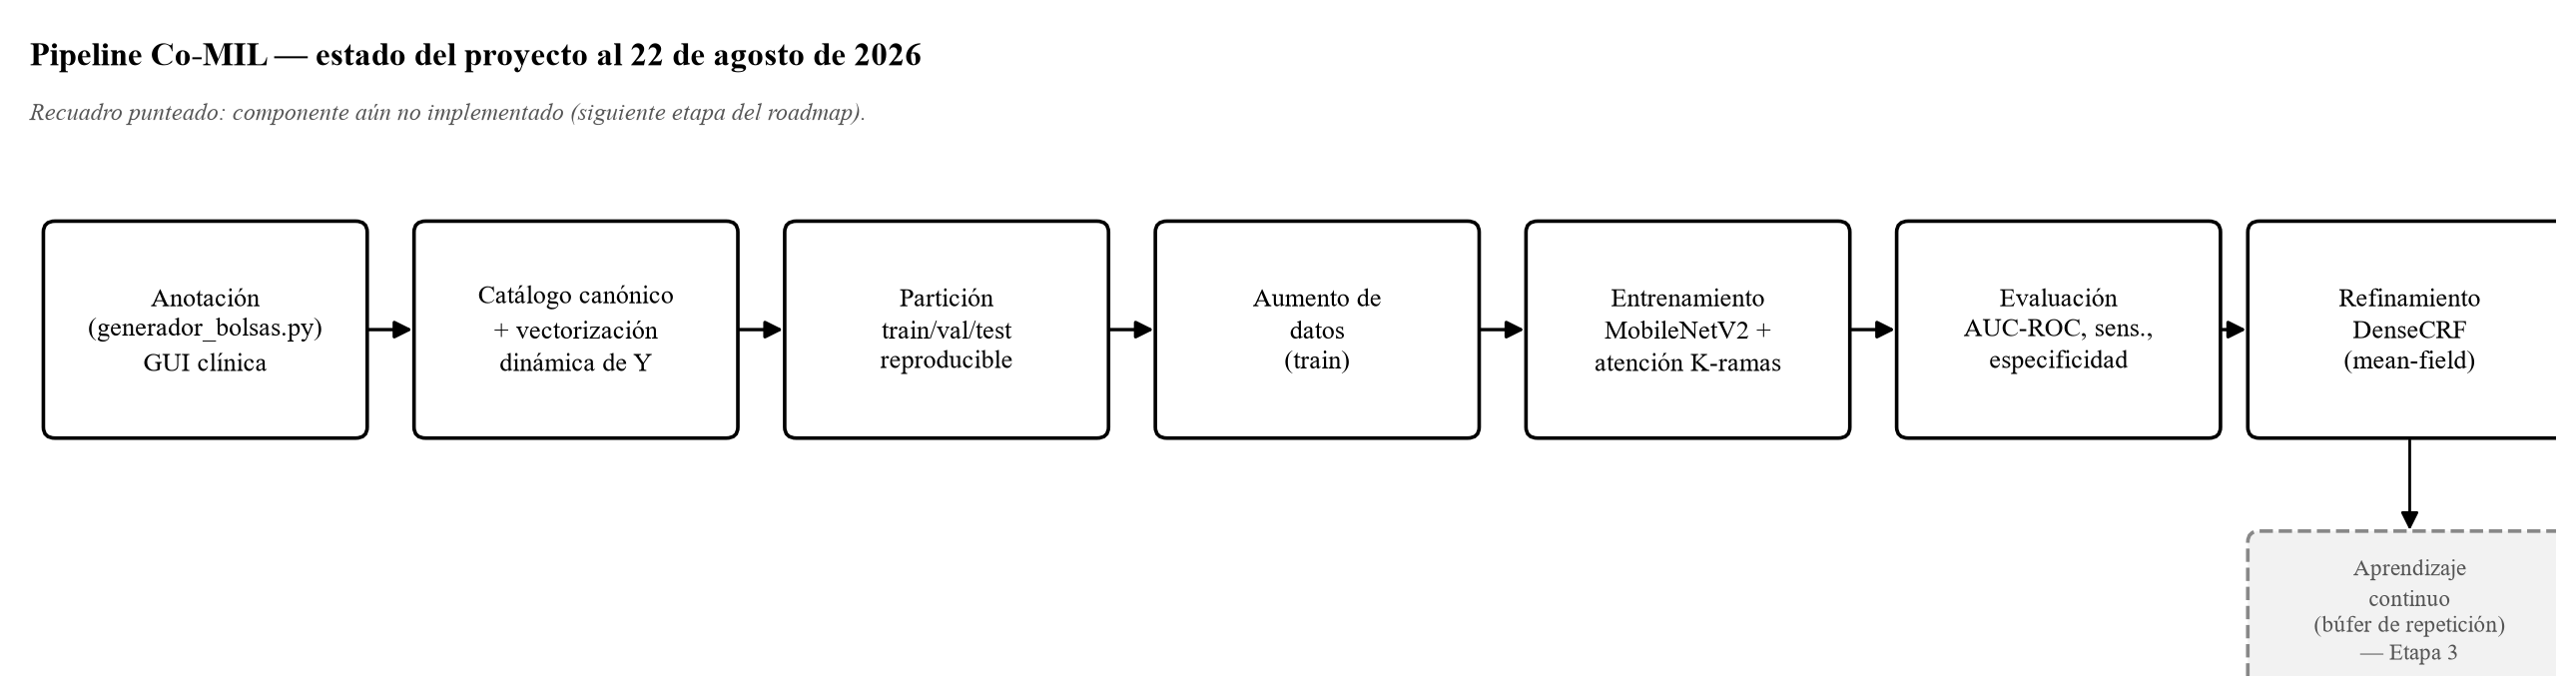
\includegraphics[width=\textwidth]{figuras/fig_pipeline_estado_actual.png}
\caption{Pipeline completo de Co-MIL al 22 de agosto de 2026. El recuadro punteado (aprendizaje
continuo) es la única etapa mayor del plan de tesis todavía sin implementar.}
\label{fig:pipeline}
\end{figure}

\begin{figure}[H]
\centering
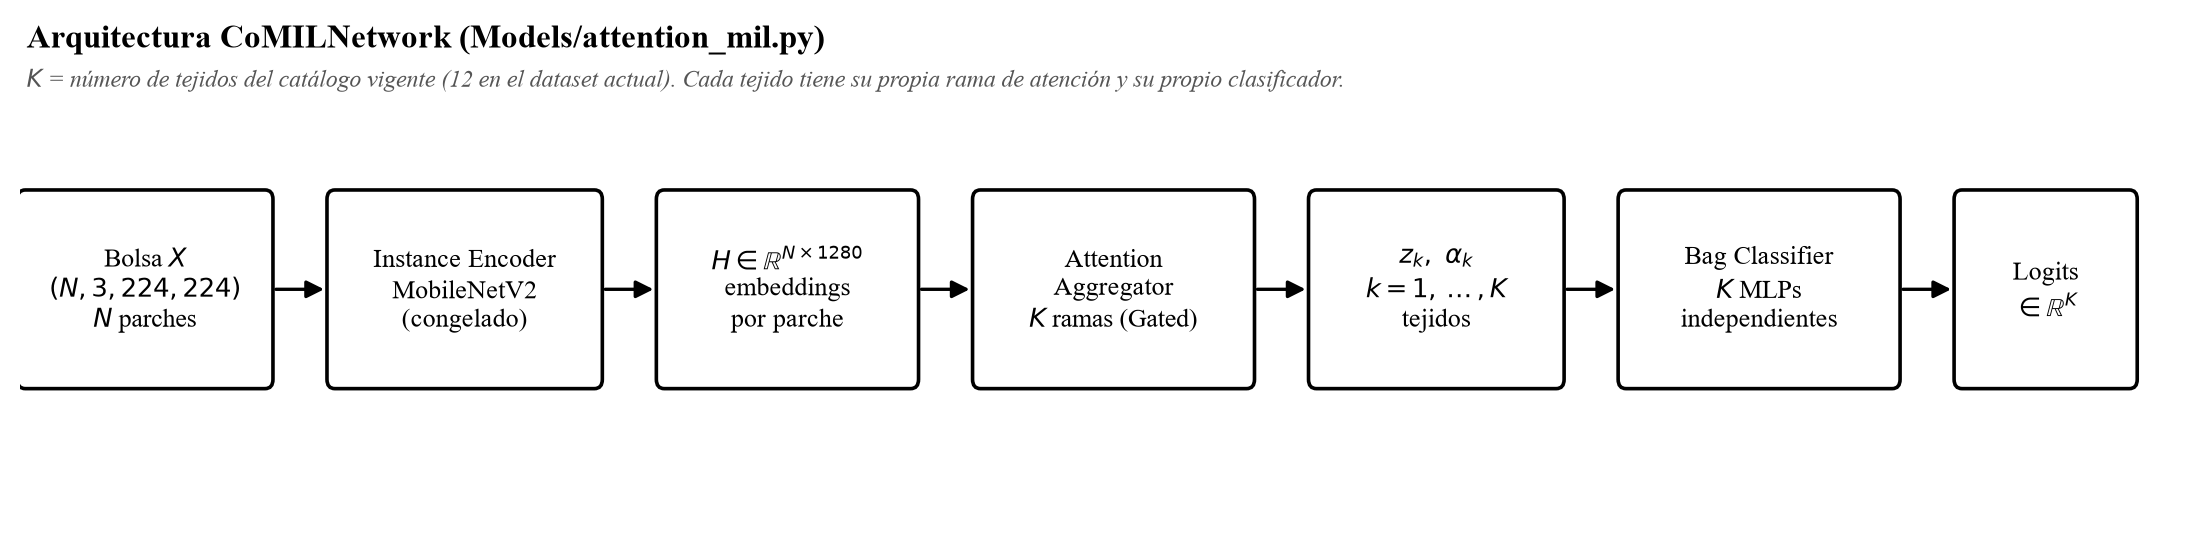
\includegraphics[width=\textwidth]{figuras/fig_arquitectura_modelo.png}
\caption{Arquitectura \texttt{CoMILNetwork}: MobileNetV2 congelado como extractor de
características, seguido de $K$ ramas de atención independientes (una por tejido) y $K$
clasificadores MLP independientes.}
\label{fig:arquitectura}
\end{figure}

\begin{figure}[H]
\centering
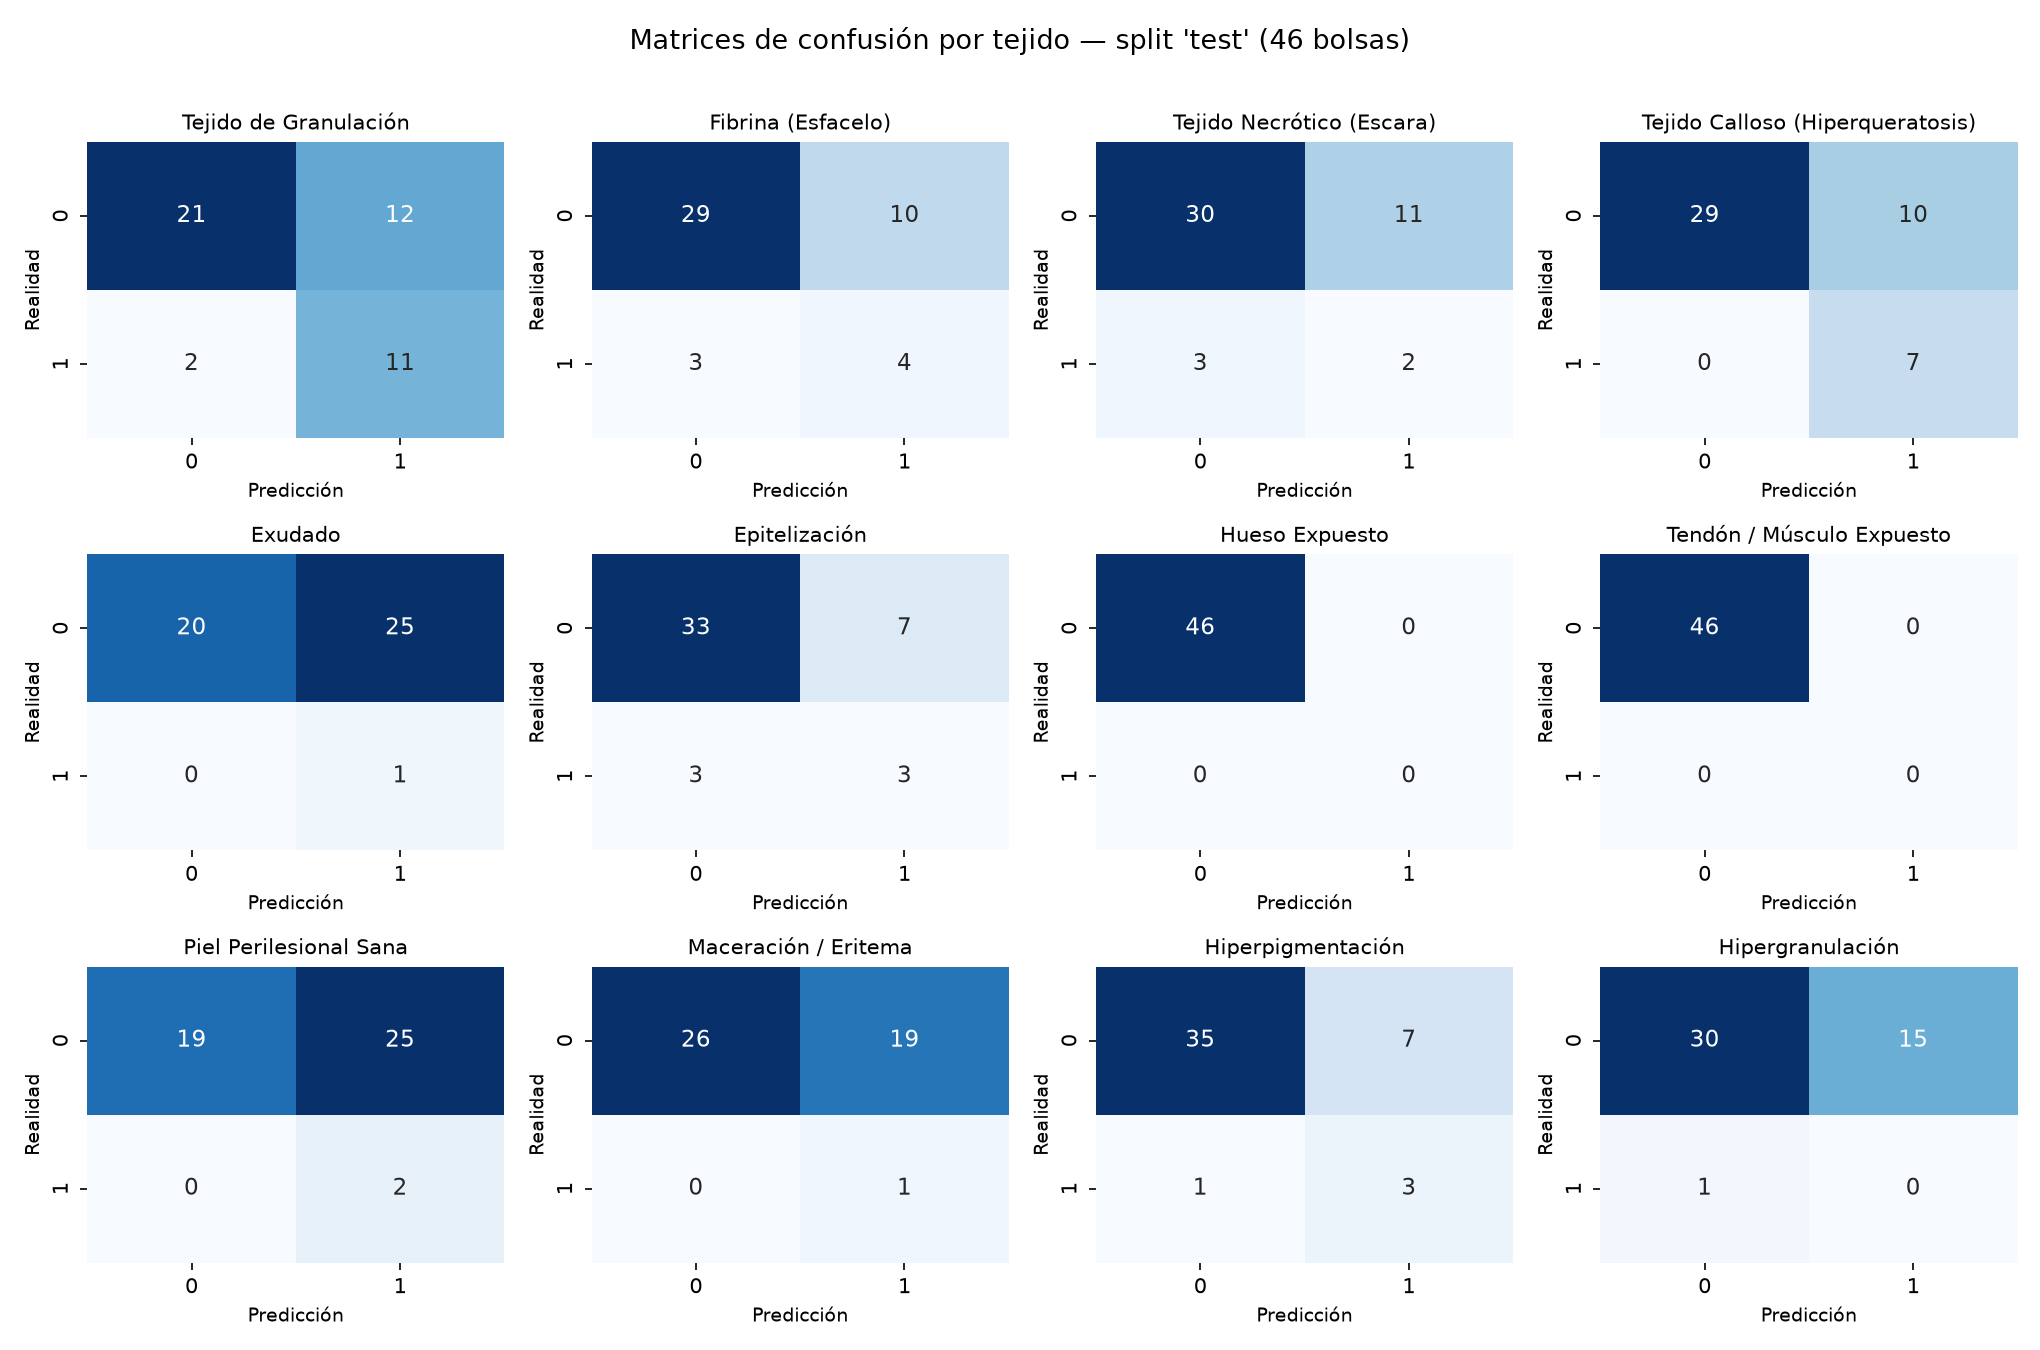
\includegraphics[width=\textwidth]{figuras/fig_matrices_confusion_test.png}
\caption{Matrices de confusión por tejido sobre el split de prueba (46 bolsas), modelo
reentrenado con la partición corregida.}
\label{fig:matrices}
\end{figure}

\begin{figure}[H]
\centering
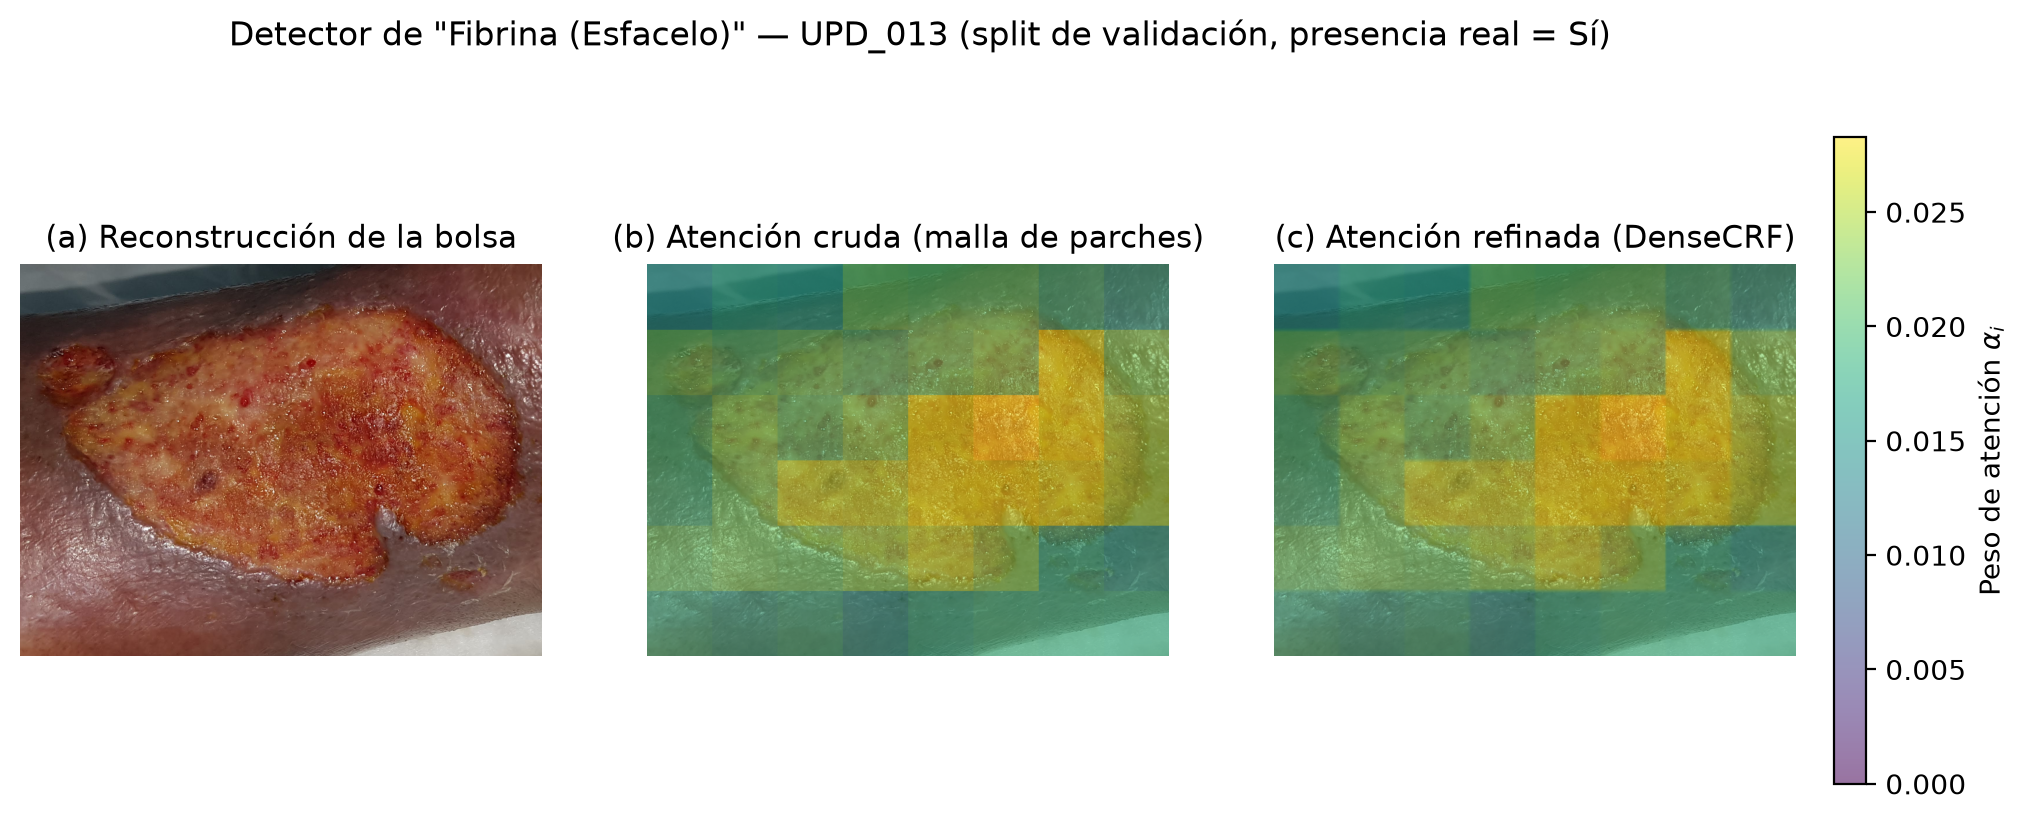
\includegraphics[width=0.95\textwidth]{figuras/fig_refinamiento_crf_fibrina.png}
\caption{Ejemplo real (split de validación, imagen UPD\_013, tejido ``Fibrina (Esfacelo)'') del
efecto del refinamiento DenseCRF: (a) reconstrucción de la bolsa, (b) atención cruda a nivel de
parche, (c) atención refinada. El efecto es sutil en este caso porque la atención cruda del modelo
todavía está poco concentrada (rango $\sim$0.015--0.028 sin picos claros) --- esperable con solo 30
épocas de entrenamiento y tan pocos datos; se espera un efecto más marcado conforme el modelo
converja mejor.}
\label{fig:crf-ejemplo}
\end{figure}

\entrada{Discusión: granularidad espacial de los mapas de atención}{Misma pregunta que el autor
dejó planteada desde el inicio de esta bitácora, retomada explícitamente hoy.}

El heatmap actual tiene, como máximo, un valor por parche de 224$\times$224 px --- para una ROI de
pocos cientos de píxeles esto deja una malla de 2$\times$2 o 3$\times$3 celdas, insuficiente para
interpretación clínica fina de bordes de tejido. Dos rutas, complementarias, ambas ya sustentadas
en el diseño existente del pipeline (no requieren rediseño desde cero):

\begin{enumerate}[leftmargin=1.5em]
    \item \textbf{Refinamiento DenseCRF} (implementado hoy, ver arriba): barato, no requiere
        reprocesar datos ni más cómputo de entrenamiento.
    \item \textbf{Parches más finos}: \texttt{reprocesador\_dataset.py} ya sabe re-extraer bolsas a
        56 o 112 px en vez de 224 px desde la imagen original en alta resolución, y
        \texttt{dataset.py} ya reescala esos parches chicos a 224 px solo para la entrada del CNN,
        conservando la malla fina para el mapa de atención. Requiere primero que
        \texttt{reprocesador\_dataset.py} propague \texttt{roi\_labels} (pendiente, ver Etapa 0 del
        roadmap), y es más caro en cómputo --- probablemente necesite GPU/Colab.
\end{enumerate}

Con esto se da por cerrada la sesión de trabajo del 22 de agosto de 2026. Próxima entrada: Etapa 3
del roadmap (diseño e implementación mínima de un búfer de repetición para el componente de
aprendizaje continuo).

% -----------------------------------------------------------------------------------
% Plantilla para futuras entradas. Copiar el bloque \entrada{...}{...} según se necesite
% dentro de una nueva \section{DD de mes de AAAA} para cada sesión de trabajo nueva.
% -----------------------------------------------------------------------------------

\end{document}
